\section{Weights}
\label{sec:weights}

In this section, we introduce several weights for the MF model. We first present two query-dependent weights: 
\begin{inparaenum}[(1)]
  \item the \emph{Query Coverage} weight which indicates how well the query terms are covered by an entity, an attribute or a value; and
  \item the \emph{Leaf Coverage} weight which indicates how well a value node is covered by a query.
\end{inparaenum}
Next, we describe the \emph{Attribute} and \emph{Entity Labels} query-independent weights.

\subsection{The Query Coverage Weight}
\label{sec:kw-factor}

The purpose of the Query Coverage (QC) weight is to lower the importance given to an entity, an attribute or a value with respect to the number of query terms it covers. This weight is combined with the ranking function using the parameters $\alpha_e$, $\alpha_a$ and $\alpha_v$. For example, given a query composed of three terms, if a value contains only occurrences of one query term, this value will then weight less than a value containing occurrences of more than one query term.\\

This weight integrates the IDF weight of query terms so that the coverage takes into account the importance of the terms it covers. For example, if two entities have occurrences of one of the three query terms, the coverage would then be $\frac{1}{3}$ for both. Thanks to the IDF weights, the entity with the more important term will have a higher coverage weight than the other one.
The query coverage weight is computed as follows:
$$
QC = \frac{\sum_{t\in X \cap q}{\omega_t^2}}{\sum_{t\in q}{\omega_t^2}}
$$
where $X$ is either a value, an attribute set or the entity and $q$ is the query.

\subsection{The Leaf Coverage Weight}
\label{sec:leaf-coverage}

The Leaf Coverage (LC) weight reflects the proportion of terms in a value matching the query, i.e., how much it is covered by the query. Since a leaf in the MF ranking model holds some content about the entity, we assume that the more query terms match a large portion of the leaf, the more this leaf is a ``precise'' description of the query. This weight is integrated into the MF ranking function using the parameter $\alpha_v$.\\

The leaf coverage is defined as the quotient of the query terms frequencies in the leaf over its \emph{leaf length}:
$$
LC = \frac{\sum_{t\in v \cap q}{F_t}}{l}
$$
where $q$ is the query, $F_t$ is the frequency of the term $t$ in the leaf $v$, and $l$ the leaf length.
However, we remark that this definition disadvantages longer values over shorter ones in the case where the sum of term frequencies is equal. Indeed, given a query with two terms which occur $x$ times in total within two leaves, the small leaf with occurrences of one term would receive a higher weight than the larger leaf with occurrences of the two; this is due to the division by the \emph{leaf length} $l$.\\

\begin{figure}
	\centering
	\definecolor{myblue}{cmyk}{20,10,0,0}
	\begin{subfigure}{.45\textwidth}
		\centering
		\resizebox{\textwidth}{!}{
			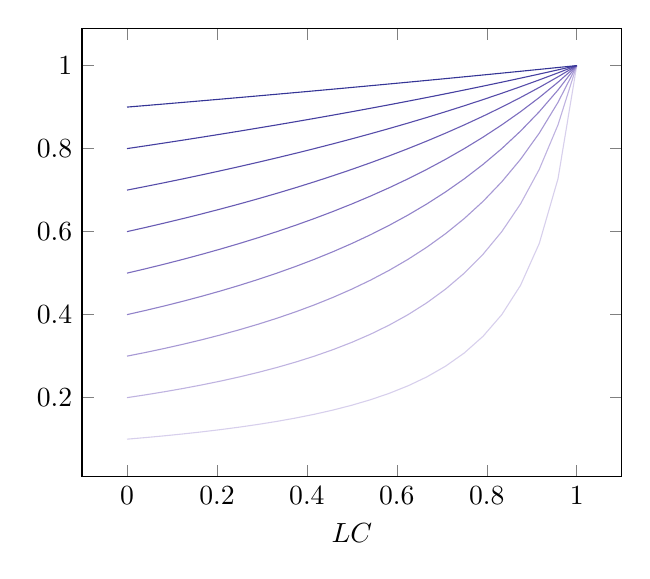
\begin{tikzpicture}
			\begin{axis}[
				xlabel=$LC$
			]
			\foreach \alpha in {1,...,9}
			{
				\pgfmathsetmacro\k{\alpha*10+5}
				\edef\tmp{\noexpand\addplot[myblue!\k][domain=0:1]}
				\tmp {(\alpha/10) / (1 + ((\alpha/10) - 1) * x^1)};
			}
			\end{axis}
			\end{tikzpicture}
		}
		\caption{The parameter $\alpha$ varies from $0.1$ to $0.9$}
	\end{subfigure}
	\qquad
	\begin{subfigure}{.45\textwidth}
		\centering
		\resizebox{\textwidth}{!}{
			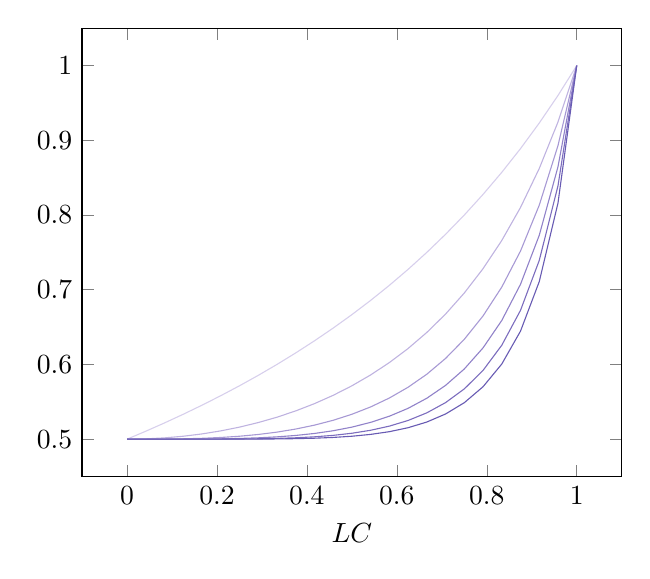
\begin{tikzpicture}
			\begin{axis}[
			xlabel=$LC$
			]
			\foreach \n in {1,...,6}
			{
				\pgfmathsetmacro\k{\n*10+5}
				\edef\tmp{\noexpand\addplot[myblue!\k][domain=0:1]}
				\tmp {.5 / (1 - 0.5 * x^\n)};
			}
			\end{axis}
			\end{tikzpicture}
		}
		\caption{The parameter $n$ varies from $1$ to $6$}
	\end{subfigure}
	\caption{Effect of the control function over the LC coverage. The opacity of the curve gets stronger as the parameter increases.}
	\label{fig:control-function}
\end{figure}

In order to have a better control over the effect of the LC weight, we developed a \emph{control} function which
\begin{inparaenum}[(1)]
	\item imposes a fixed lower bound $\alpha$ to prevent short values receiving a higher weight than long ones; and
	\item increases as a power function with $n$ to ensure a high coverage weight only when the leaf coverage LC is close to 1.
\end{inparaenum}
\begin{equation}
\label{eq:lc-norm}
\frac{\alpha}{1+(\alpha-1)\times LC^n}
\end{equation}
where $\alpha \in \; ]0,1[$ is a parameter that sets the lower bound of LC, and $n$ is a parameter that controls the effect of the coverage on the leaf. Figure~\ref{fig:control-function} depicts effects of the two parameters $\alpha$ and $n$ over the leaf coverage LC. We can see that the higher $n$ is, the higher the coverage needs to be for the leaf to receive a weight higher than $\alpha$.

\subsection{The Attribute and Entity Labels Weights}
\label{sec:att-subj-w}

The Attribute and Entity Labels (AEL) weights balance the importance of an entity or an attribute depending on its label. This weight is integrated into the ranking function using the $\alpha_a$ parameter.
The weight value is defined empirically, and depends on the attribute. For instance, in a dataset concerned about books, a query match on the title might be considered more important than a match on the author's description.
